\documentclass[aspectratio=169]{beamer}
   \usetheme{metropolis}
   \setbeamertemplate{blocks}[rounded][shadow=false]
\usepackage{url}
\usepackage{hyperref}
\usepackage{booktabs}
\usepackage{tabularx}
\usepackage{dcolumn}
   \newcolumntype{d}[1]{D{.}{.}{#1}}
\usepackage{graphicx}
\usepackage{adjustbox}
\usepackage{color}
\usepackage{textpos}
\usepackage{etoolbox}
\usepackage[super]{nth}
\usepackage[cache=false]{minted}

\makeatletter
\patchcmd{\beamer@sectionintoc}{\vskip1.5em}{\vskip0.5em}{}{}
\makeatother

\definecolor{smured}{rgb}{0.797,0,0.027}
\definecolor{smublue}{RGB}{48,64,116}
\definecolor{dkgreen}{rgb}{0,0.6,0}
\definecolor{gray}{rgb}{0.5,0.5,0.5}
\definecolor{mauve}{rgb}{0.58,0,0.82}
\definecolor{text_gray}{RGB}{46,58,62}

\setbeamercolor{progress bar}{fg=smured,bg=smublue}
\setbeamercolor{title separator}{fg=smublue}
\setbeamercolor{frametitle}{bg=smublue}

\metroset{
  numbering=fraction
}

\hypersetup{
  colorlinks=true,
  allcolors=text_gray,
  urlcolor=smured,
}

\addtobeamertemplate{frametitle}{}{
\begin{textblock*}{1cm}(\textwidth,-1.155cm)

\includegraphics[width=1cm]{figures/smu_logo.pdf}
\end{textblock*}}

\setminted{breaklines,linenos,fontsize=\scriptsize}
\setmintedinline{fontsize=auto}

\title{Introduction to Standard C++ Parallel Algorithms}
\author{Robert Kalescky\\ HPC Applications Scientist}
\institute{
Research and Data Sciences Services\\
Office of Information Technology\\
Center for Research Computing\\
Southern Methodist University}
\date{April 28, 2021}

\begin{document}

\begin{frame}
\titlepage
\end{frame}

\begin{frame}{Outline}
\footnotesize
\tableofcontents[hideallsubsections]
\end{frame}

\section{Research Support}

\begin{frame}{Research and Data Science Services}
\begin{itemize}
  \item Provide research computing support, consultations, and collaborations
  \item Data Science - Dr. Eric Godat
  \item High-Performance Computing - Dr. Robert Kalescky \& Dr. John LaGrone
  \item Custom Devices (IOT, wearables, etc.) - Guillermo Vasquez
\end{itemize}
\end{frame}

\begin{frame}{Center for Research Computing (CRC)}
\begin{itemize}
  \item Maintains our primary shared resource for research computing, ManeFrame II (M2), in collaboration with OIT
  \item Provides research computing tools, support, and training to all faculty, staff, and students using research computing resources
  \item \url{www.smu.edu/crc} has documentation and news
  \item \href{mailto:help@smu.edu}{help@smu.edu} or \href{mailto:rkalescky@smu.edu}{rkalescky@smu.edu} for help
  \item Request an account at \url{www.smu.edu/crc}
\end{itemize}
\end{frame}

\begin{frame}{Spring 2022 CRC HPC Workshop Series}
\begin{table}
\tiny
\begin{tabular}{lll}
Date     & Time  & Workshop\\
\hline
February 2 & 2-4 & ManeFrame II (M2) Introduction \\  
February 9 & 2-4 & Workflows in R \\  
February 15 & 3-5 & Finding and Preparing Text Data Sets for Mining \\
Febryary 16 & 1-4 & Machine Learning with Python Part 1 \\
February 17 & 12-1 & AI for the Non-Expert \\
February 18 & 12-1 & Introduction to GitHub \\        
February 23 & 2-4  & Containers and Spack \\     
March 2   &  2-4 &  ManeFrame II (M2) Introduction \\
March 3   &  1-4 & Data Science Workflow with R \\  
March 8   &  3-6 & Introduction to Python for Text Mining \\ 
March 9   &  1-4 & Machine Learning with Python Part 2 \\ 
March 22  &  3-6 & Getting Support for Text Mining \\  
March 23  &  2-4 & Shared Memory Parallelism \\   
March 30  &  1-4 & Deep Learning with Python Part 1 \\   
April 6   &  2-4 & ManeFrame II (M2) Introduction \\    
April 13  &  2-4 & Accelerator Libraries and APIs \\    
April 20  &  1-4 & Deep Learning with Python Part 2 \\      
April 27  &  2-4 & MPI/NCCL/SHMem \\            
May 4     &  2-4 & ManeFrame II (M2) Introduction      
\end{tabular}
\caption{Workshops will be held each Wednesday from 2:00 to 4:00 PM. Sessions will typically be                                
recorded and posted along with session materials.         
Register on the Library Workshop Calendar \href{https://libcal.smu.edu/calendar/libraryworkshops}{https://libcal.smu.edu/calendar/libraryworkshops}
}
\end{table}
\end{frame}

\section{ManeFrame II (M2)}

\begin{frame}{Cluster Super Computers}
\begin{figure}
  \centering
  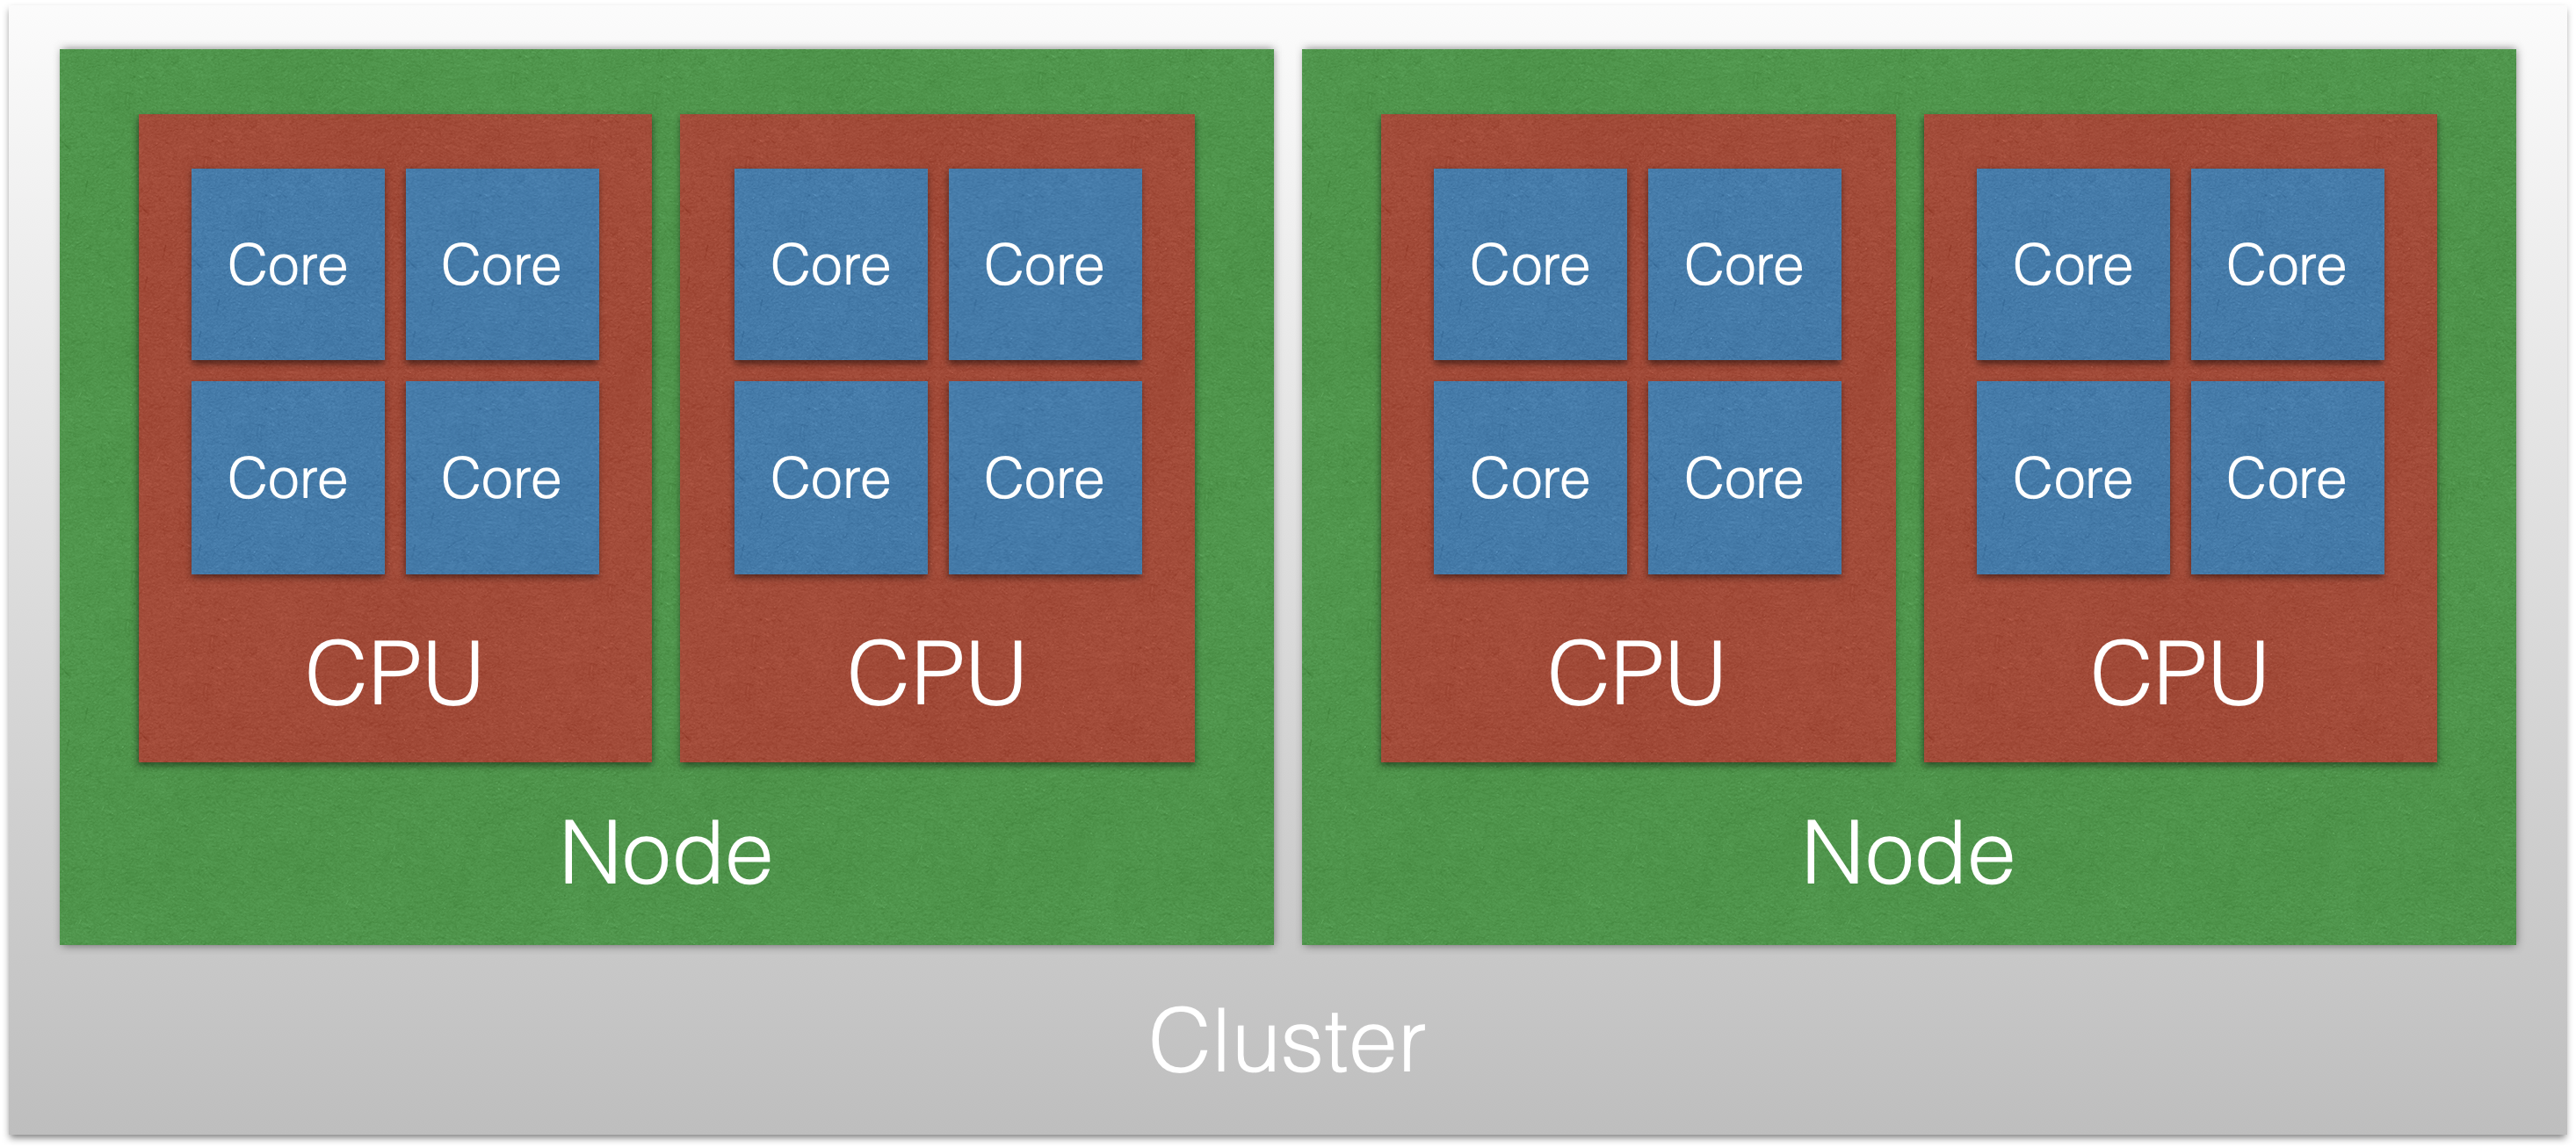
\includegraphics[width=0.75\linewidth]{figures/cluster.png}
  \caption{A cluster is a collection of individual computers networked together. Applications can be configured to run on all available compute resources.}
\end{figure}
\end{frame}

\begin{frame}{ManeFrame II (M2) Node Types}
\begin{table}
\tiny
\begin{tabular}{lllll}
\toprule
Type & Quantity & Cores & Memory [GB] & Additional Resources\\
\midrule
Standard-Memory & 176 & 36 & 256 & \\
Medium-Memory-1 & 35 & 36 & 768 & \\
Medium-Memory-2 & 4 & 24 & 768 & 3 TB SSD local scratch\\
High-Memory-1 & 5 & 36 & 1,536 & \\
High-Memory-2 & 6 & 40 & 1,536 & 3 TB SSD local scratch\\
GPGPU-1 & 36 & 36 & 256 & NVIDIA P100 GPU has 3,584 CUDA cores and 16 GB CoWoS\\
MIC-1 & 36 & 64 & 384 & 16 GB of high bandwidth (400 GB/s) stacked memory\\
VDI & 5 & 36 & 256 & NVIDIA Quadro M5000 GPU\\
v100x8 & 3 & 36 & 768 & 8 NVIDIA V100 GPUs with 5,120 CUDA cores and 32 GB CoWoS\\
Faculty Partner Nodes & 3 &  &  & Various research specific NVIDIA GPU configurations\\
\midrule
ManeFrame II & 354 & 11,276 & 120 TB & 2.8 PB storage and InfiniBand network\\
\bottomrule
\end{tabular}
\end{table}
\end{frame}

\begin{frame}{ManeFrame II (M2) Partitions (Queues)}
\begin{table}
\tiny
\begin{tabular}{llll}
\toprule
Partition & Duration & Cores & Memory [GB]\\
\midrule
development & 2 hours & various & various\\
htc & 1 day & 1 & 6\\
standard-mem-s & 1 day & 36 & 256\\
standard-mem-m & 1 week & 36 & 256\\
standard-mem-l & 1 month & 36 & 256\\
medium-mem-1-s & 1 day & 36 & 768\\
medium-mem-1-m & 1 week & 36 & 768\\
medium-mem-1-l & 1 month & 36 & 768\\
medium-mem-2 & 2 weeks & 24 & 768\\
high-mem-1 & 2 weeks & 36 & 1538\\
high-mem-2 & 2 weeks & 40 & 1538\\
mic & 1 week & 64 & 384\\
gpgpu-1 & 1 week & 36 & 256\\
v100x8 & 1 week & 1 & 20\\
fp-gpgpu-2 & various & 24 & 128\\
fp-gpgpu-3 & various & 40 & 384\\
\bottomrule
\end{tabular}
\end{table}
\end{frame}

\begin{frame}{ManeFrame II File Systems}
\begin{description}
\item[\$HOME]
\begin{itemize}
  \item Default file system when logging into M2, e.g. \mintinline{sh}{/users/$USER}.
  \item Space should be used to write, edit, compile programs, and job submission scripts, etc.
  \item Restricted by quotas (200 GB) and backed-up.
\end{itemize}
\item[\$WORK]
\begin{itemize}
  \item Long term storage at \mintinline{sh}{/work/users/$USER}.
  \item Restricted by quotas (8 TB) and not backed-up.
\end{itemize}
\item[\$SCRATCH]
\begin{itemize}
 \item Scratch space at \mintinline{sh}{/scratch/users/$USER}.
 \item Treat \$SCRATCH as a volatile file system that is not backed-up.
 \item Beginning October 1, 2021, \mintinline{sh}{$SCRATCH} has a 60-day retention policy, i.e. untouched files will be removed after 60 days.
\end{itemize}
\end{description}
\end{frame}



\section{C++ Parallel Algorithms}

%\begin{frame}{}
%\begin{itemize}
%  \item 
%\end{itemize}
%\end{frame}

\begin{frame}{C++ Parallel Algorithms}
\begin{itemize}
  \item C++17 introductions high-level parallel versions of many algorithms
        found in the Standard Template Library
  \item Several new algorithms were included specifically to aid in using the
        new parallel algorithms, \textit{e.g.} \mintinline{c++}{std::reduce} and
        \mintinline{c++}{std::transform_reduce}
  \item Each parallel algorithm has an execution policy that defines how the
        algorithm is parallelized
\end{itemize}
\end{frame}

\begin{frame}{Execution Policies}
The C++17 standard defines three execution policies:
\begin{description}
  \item[\mintinline{c++}{std::execution::seq}] Sequential execution, \textit{i.e.} no parallelism
  \item[\mintinline{c++}{std::execution::par}] Parallel execution via one or more threads
  \item[\mintinline{c++}{std::execution::par_unseq}] Parallel execution via one or more threads with each thread possibly vectorized
\end{description}
\end{frame}

\begin{frame}{Parallel Execution}
When using an execution policy other than \mintinline{c++}{std::execution::seq}:
\begin{itemize}
  \item The compiler \textbf{may} execute the algorithm in parallel when possible and advantageous (some conforming C++17 inplementations may ignore the parallelization flag and run via \mintinline{c++}{std::execution::seq})
  \item It is up to \textbf{you} to make sure that the algorithm and data are safe to be run in parallel
\end{itemize}
\end{frame}

\begin{frame}{Additional Resources}
\begin{itemize}
  \item \href{https://en.cppreference.com/w/cpp/algorithm}{C++ STL Algorithms Documentation}
  \item \href{https://docs.nvidia.com/hpc-sdk/compilers/c++-parallel-algorithms/index.html}{NVIDIA HPC SDK Documentation}
  \item \href{https://livebook.manning.com/book/c-plus-plus-concurrency-in-action-second-edition/chapter-10}{C++ Concurrancy In Action, \nth{2} Edition}
  \item \href{https://www.youtube.com/watch?v=FJIn1YhPJJc}{CppCon 2018: Bryce Adelstein Lelbach ``The C++ Execution Model''}
  \item \href{https://developer.download.nvidia.com/video/gputechconf/gtc/2019/presentation/s9770-c++17-parallel-algorithms-for-nvidia-gpus-with-pgi-c++.pdf}{C++17 Parallel Algorithms on NVIDIA GPUs with PGI C++}
\end{itemize}
\end{frame}


\section{Using oneAPI On ManeFrame II (M2)}

\begin{frame}{Using oneAPI On ManeFrame II (M2)}
\begin{itemize}
  \item All Intel oneAPI compilers, libraries, and tools are made availabe on M2 via \mintinline{sh}{module load intel/oneAPI-2021.lua}
  \item \href{https://github.com/oneapi-src/oneAPI-samples}{Intel oneAPI Toolkit Samples}
\end{itemize}
\end{frame}

\begin{frame}{Components}
\begin{figure}
  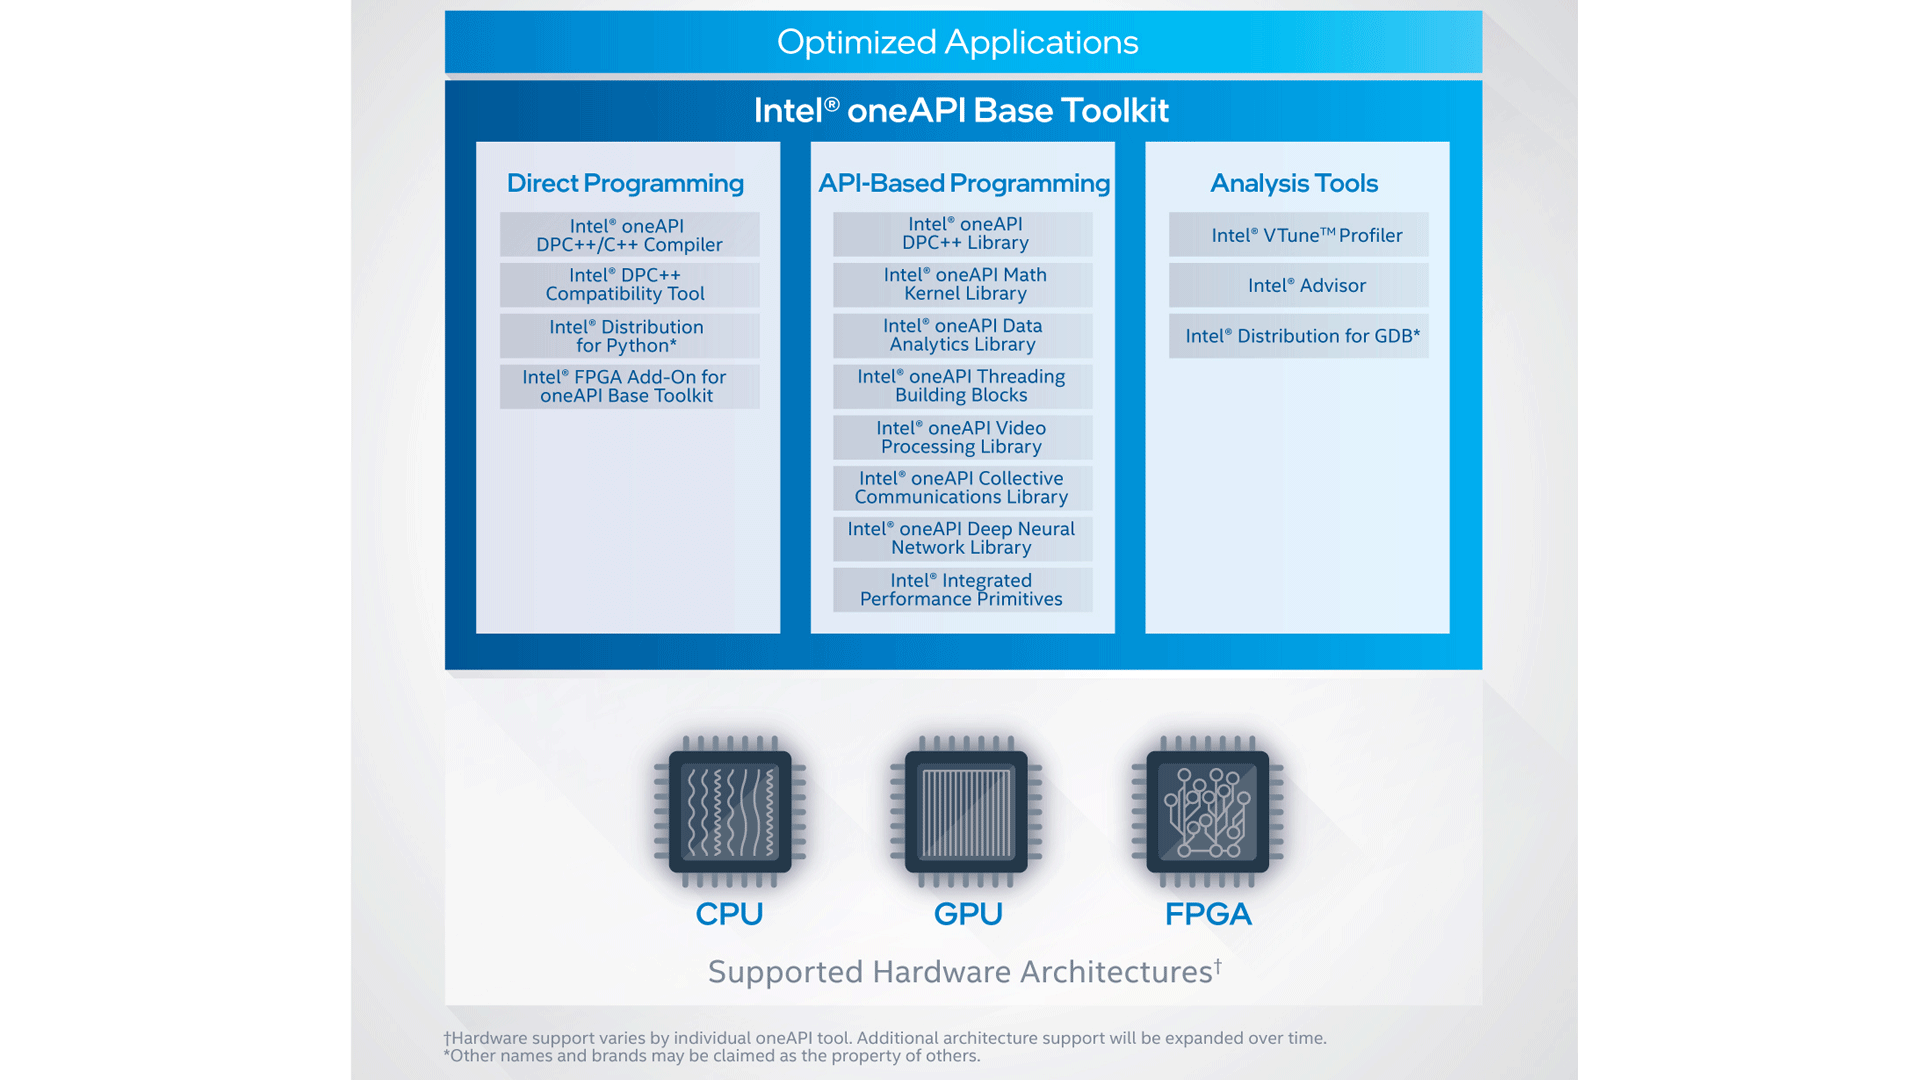
\includegraphics[width=0.75\linewidth]{figures/diagram-onapi-base-toolkit-16x9.png}
  \caption{Components of the oneAPI 2021 base installation.}
\end{figure}
\end{frame}

\subsection{Compilers}

\begin{frame}{oneAPI DPC++/C++ Compiler}
\begin{columns}
\begin{column}{0.5\textwidth}
\begin{itemize}
  \item Standards-based C++ compiler based on the open source LLVM compiler infrastructure
  \begin{itemize}
    \item Full support up through C++17
    \item Initial support for C++20
  \end{itemize}
  \item SYCL compiler
  \item DPC++ compiler (SYCL with Intel extensions)
  \item Partial support for OpenMP 4.5 and 5.0 offloading
\end{itemize}
\end{column}
\begin{column}{0.5\textwidth}
\begin{figure}
  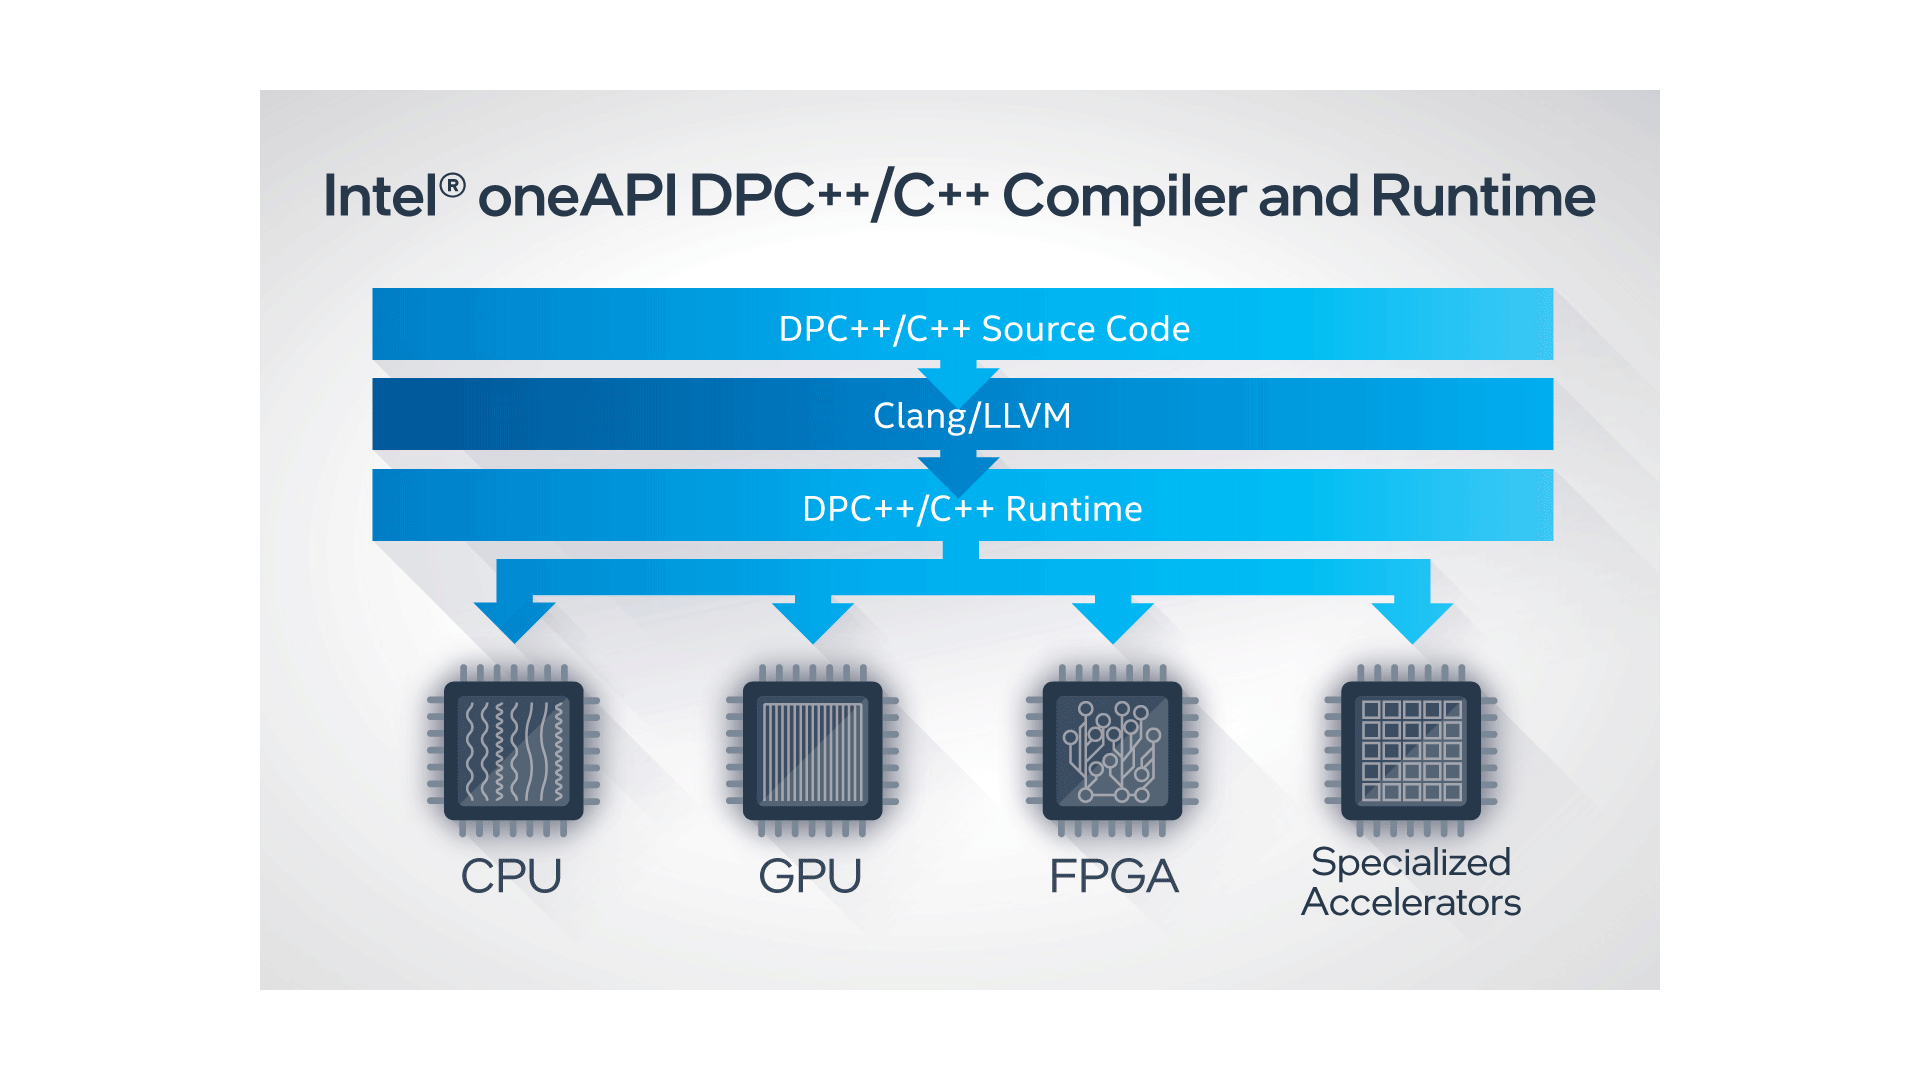
\includegraphics[width=\linewidth]{figures/diagram-oneapi-dpc-c-compiler-16x9.png}
  \caption{oneAPI DPC++ and C++ compiler and runtime.}
\end{figure}
\end{column}
\end{columns}
\end{frame}

\begin{frame}{oneAPI DPC++ Library}
\begin{itemize}
  \item Productivity APIs for heterogeneous computing
  \item Optimized standards-based and familiar APIs:
  \begin{itemize}
    \item C++ STL
    \item Parallel STL (PSTL)
    \item Boost.Compute
    \item Standard SYCL
  \end{itemize}
  \item Custom iterators for parallel algorithms
  \item Use device and host containers to target GPUs and FPGAs or run your code across multi-node CPUs
\end{itemize}
\end{frame}

\begin{frame}{oneAPI Threading Building Blocks}
\begin{itemize}
  \item Simplifies the work of adding parallelism to complex applications
  \item Runtime library automatically maps logical parallelism onto threads, making more efficient use of node resources
  \item Scalable data-parallel programming
    \begin{itemize}
    \item Multiple threads to work on different parts of a collection
    \item Scales well to larger numbers of processors by dividing the collection into smaller pieces
    \item Program performance increases as processors and accelerators are added
  \end{itemize}
\end{itemize}
\end{frame}

\begin{frame}{Intel Advisor}
\begin{itemize}
  \item Design and analysis tool for achieving high application performance
  \item Helps identify efficient threading, vectorization, and memory use, and GPU offload
  \item Supports C, C++, Fortran, DPC++, OpenMP, and Python.
  \item Intel Advisor features:
  \begin{itemize}
    \item Offload Advisor
    \item Automated Roofline Analysis
    \item Vectorization Advisor
    \item Threading Advisor
    \item Flow Graph Analyzer
  \end{itemize}
\end{itemize}
\end{frame}

\begin{frame}{Intel VTune Profiler}
\begin{columns}
\begin{column}{0.5\textwidth}
\begin{itemize}
  \item Application performance profiler for CPU, GPU, and FPGA
  \item Supports DPC++, C, C++, Fortran, OpenCL, Python, assembly, or any combination
  \item Get coarse-grained system data for an extended period or detailed results mapped to source code.
  \item Low system overhead
\end{itemize}
\end{column}
\begin{column}{0.5\textwidth}
\begin{figure}
  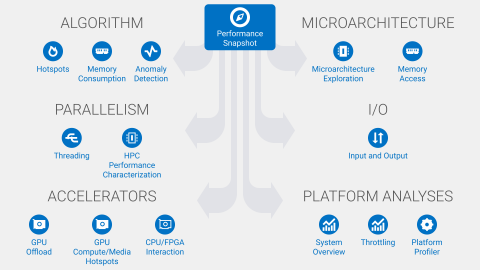
\includegraphics[width=\linewidth]{figures/diagram-vtune-bigpicture-16x9.png}
  \caption{Intel VTune Profiler overview.}
\end{figure}
\end{column}
\end{columns}
\end{frame}

\begin{frame}{Intel Inspector}
\begin{itemize}
  \item Helps find memory errors and nondeterministic threading errors and problems
  \item Dynamic memory and threading error debugger for C, C++, and Fortran applications
\end{itemize}
\end{frame}

\begin{frame}{Intel Trace Analyzer and Collector}
\begin{itemize}
  \item Profiles and analyzes MPI applications
  \item Discover temporal dependencies and bottlenecks
  \item Check the correctness of your application
  \item Locate potential programming errors, buffer overlaps, and deadlocks
  \item Visualize and understand parallel application behavior
  \item Evaluate profiling statistics and load balancing
  \item Analyze performance of subroutines or code blocks
  \item Learn about communication patterns, parameters, and performance data
  \item Identify communication hot spots
  \item Decrease time to solution and increase application efficiency
\end{itemize}
\end{frame}

\subsection{Further Information}

\begin{frame}{Further Information}
\begin{itemize}
  \item \href{https://www.oneapi.com}{The oneAPI Specification}
  \item \href{https://www.apress.com/gp/book/9781484255735}{Data Parallel C++ (Free eBook)}
  \item \href{https://software.intel.com/content/www/us/en/develop/tools/oneapi/base-toolkit.html}{Intel oneAPI Base Toolkit}
  \item \href{https://software.intel.com/content/www/us/en/develop/tools/oneapi/hpc-toolkit.html}{Intel oneAPI HPC Toolkit}
  \item \href{https://github.com/oneapi-src/oneAPI-samples}{Intel oneAPI Toolkit Samples}
\end{itemize}
\end{frame}

\section{Using the NVIDIA HPC SDK On ManeFrame II (M2)}

\begin{frame}{Using the NVIDIA HPC SDK On ManeFrame II (M2)}
\begin{itemize}
  \item All NVIDIA HPC SDK compilers, libraries, and tools are made availabe on M2 via \mintinline{sh}{module load nvhpc-21.2}
  \item \href{https://docs.nvidia.com/hpc-sdk/index.html}{NVIDIA HPC SDK Documentation}
\end{itemize}
\end{frame}

\begin{frame}{Components}
\begin{figure}
  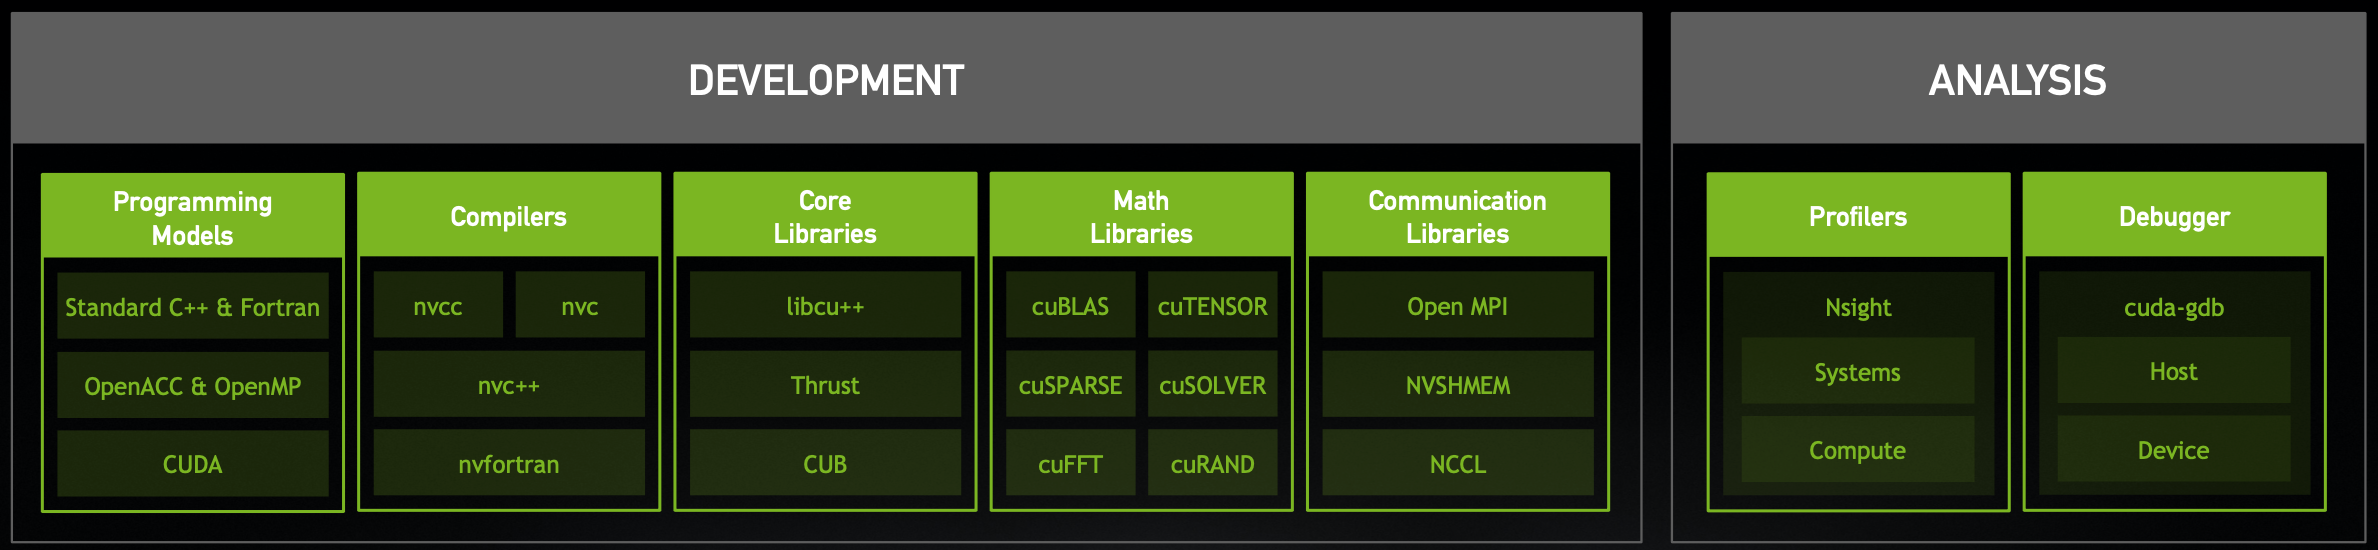
\includegraphics[width=\linewidth]{figures/nvhpc_components.png}
  \caption{Components of the NVIDIA HPC SDK.}
\end{figure}
\end{frame}

\subsection{Compilers}

\begin{frame}{NVIDIA HPC SDK Compilers}
Standards-based compilers based on the open-source LLVM compiler infrastructure.
\begin{description}
  \item[nvc] C11 compiler for NVIDIA GPUs and AMD, Intel, OpenPOWER, and Arm CPUs
  \item[nvc++] C++17 compiler for NVIDIA GPUs and AMD, Intel, OpenPOWER, and Arm CPUs
  \item[nvfortran] Fortran 2003 compiler with many Fortran 2008 featutres implemented for NVIDIA GPUs and AMD, Intel, OpenPOWER, and Arm CPUs
  \item[nvcc] CUDA C and CUDA C++ compiler driver for NVIDIA GPUs
\end{description}
\end{frame}

\subsection{Parallel Programming Models}

\begin{frame}{Parallel Programming Models}
\begin{description}
  \item[C++ -stdpar] C++ 17 Parallel Algorithms introduce parallel and vector concurrency through execution policies
  \item[OpenACC] OpenACC directives for paralleliziation on CPUs and NVIDIA GPUs
  \item[OpenMP] OpenMP directives for paralleliziation on CPUs and NVIDIA GPUs
  \item[CUDA] C, C++, and Fortran varients of CUDA for parallelization on NVIDIA GPUs
\end{description}
\end{frame}

\begin{frame}{Parallel Programming Models}
\begin{figure}
  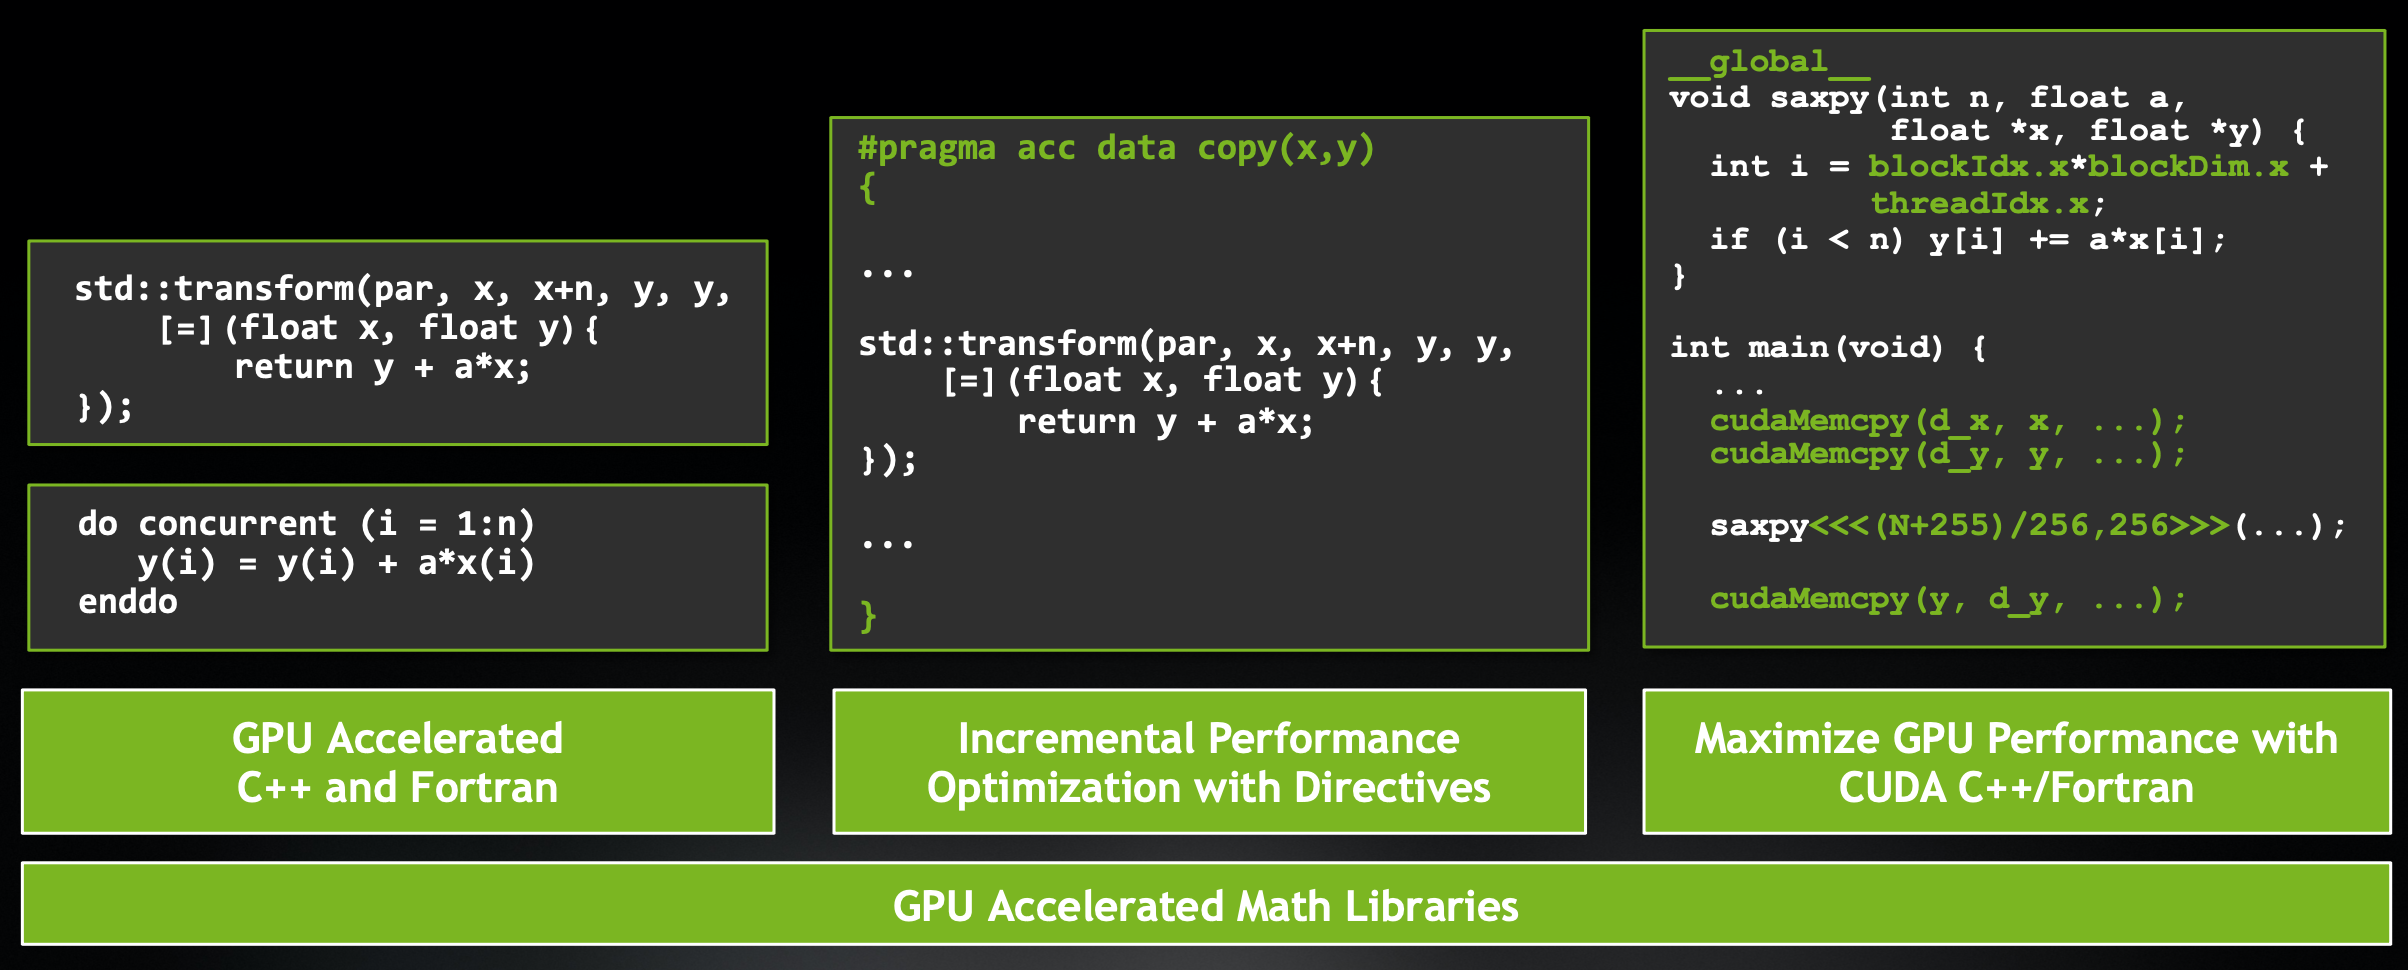
\includegraphics[width=\linewidth]{figures/use_gpu.png}
  \caption{Parallel Programming Models}
\end{figure}
\end{frame}

\begin{frame}{Parallel Programming Models}
\begin{figure}
  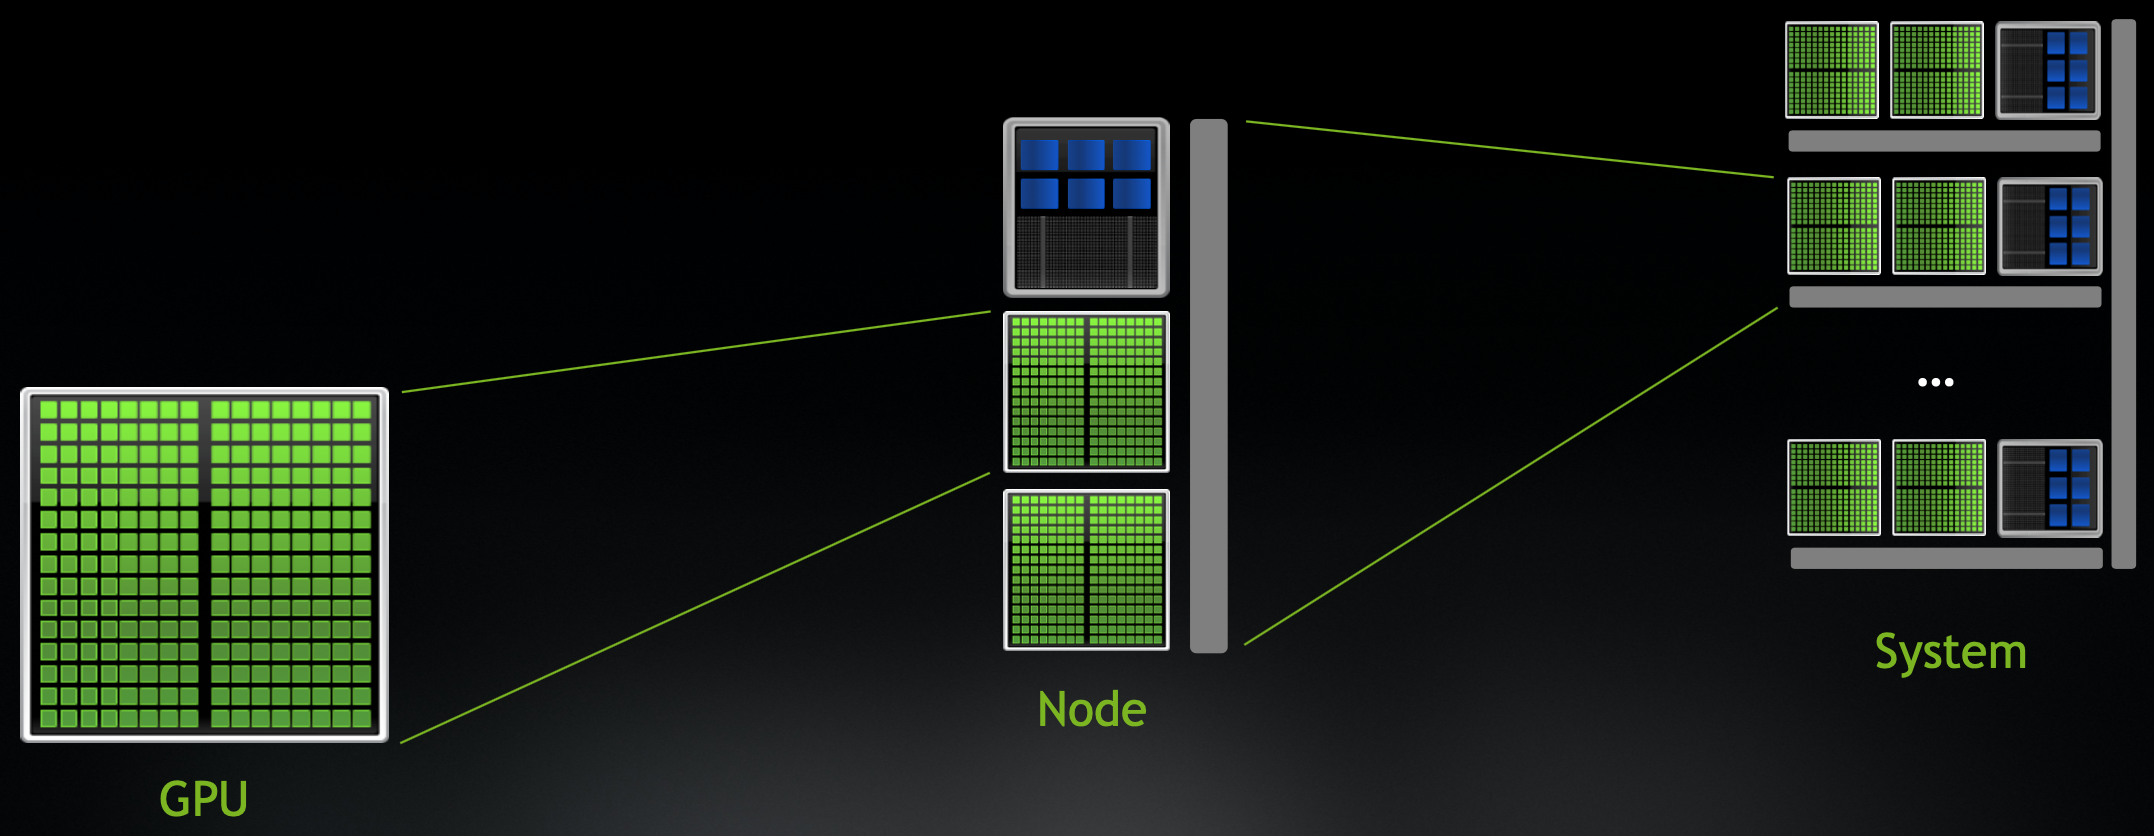
\includegraphics[width=\linewidth]{figures/parallel.png}
  \caption{Parallel Programming Models}
\end{figure}
\end{frame}

\begin{frame}{C++ Standard Parallel Algorithms (stdpar)}
\begin{figure}
  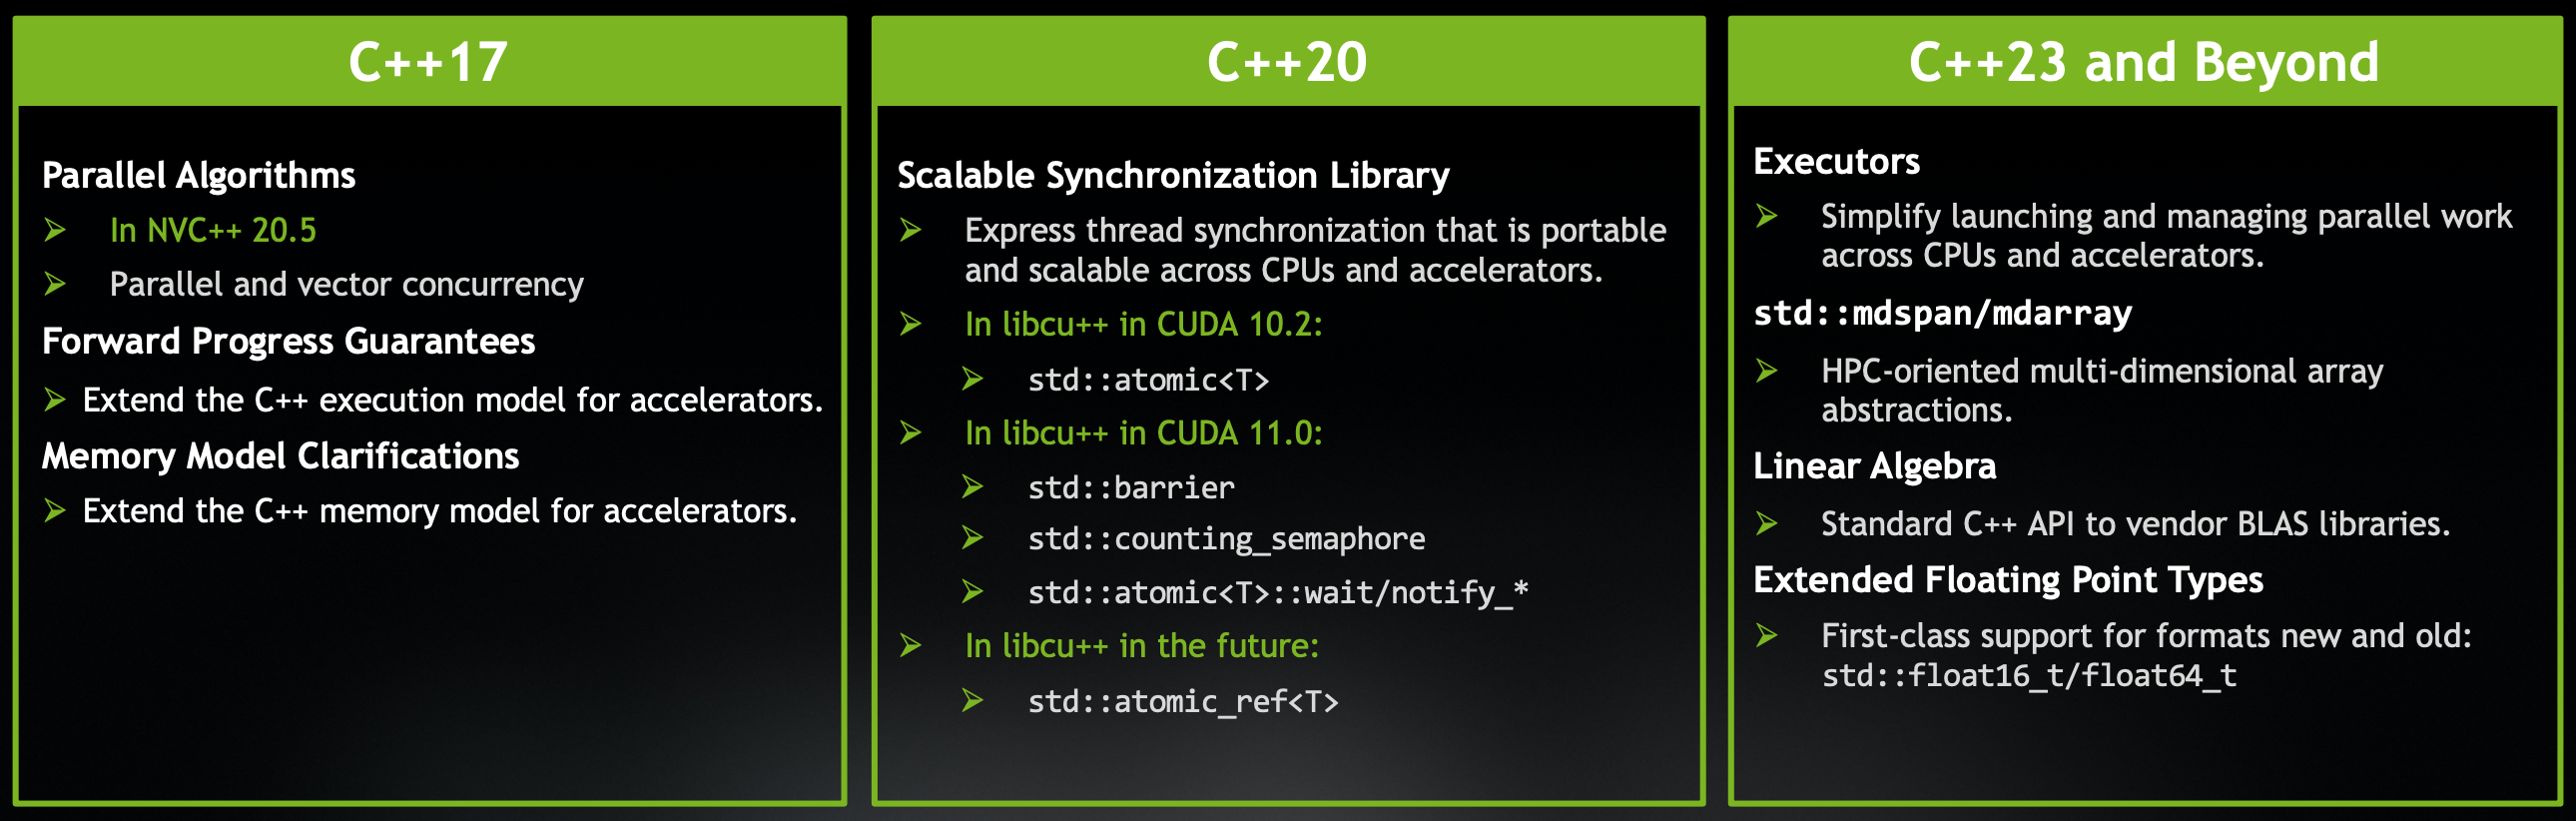
\includegraphics[width=\linewidth]{figures/cpp.png}
  \caption{Communications Libraries}
\end{figure}
\end{frame}

\begin{frame}{C++ Standard Parallel Algorithms (stdpar)}
\begin{figure}
  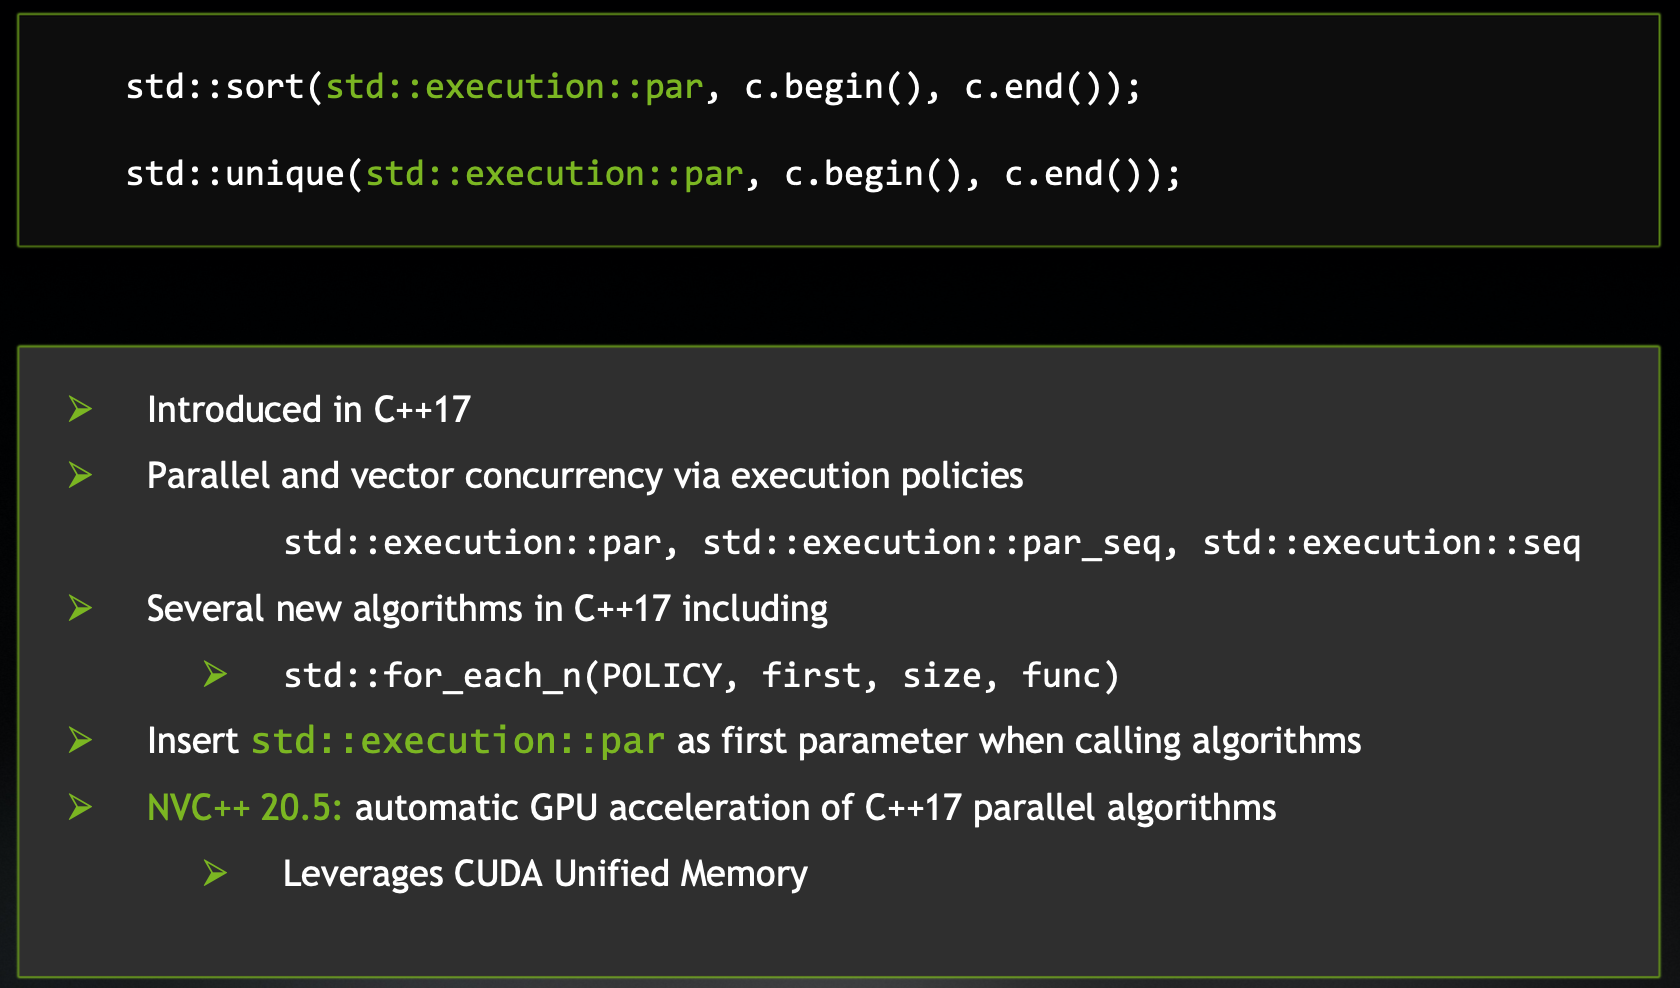
\includegraphics[height=0.75\textheight]{figures/cpp_1.png}
  \caption{Communications Libraries}
\end{figure}
\end{frame}

\subsection{Tools}

\begin{frame}{Tools}
\begin{description}
  \item[CUDA-GDB] Debugging CUDA applications.
  \item[Nsight Compute] Interactive kernel profiler for CUDA applications
  \item[Nsight System] System-wide performance analysis tool designed to visualize application algorithms
  \item[Compute Sanitizer] Functional correctness checking tools suite
  \item[NVTX] API for annotating application events, code ranges, and resources for use with Nsight
\end{description}
\end{frame}

\section{Example}

\begin{frame}{LULESH}
\begin{listing}[H]
\inputminted[firstline=3,firstnumber=1]{bash}{examples/stdpar/lulesh.sh}
\caption{Commands to build and run LULESH on ManeFrame II (M2).}
\end{listing}
\end{frame}

\begin{frame}{Help?}
\centering
Need help or have questions?\\
\href{mailto:rkalescky@smu.edu}{rkalescky@smu.edu} \\
\href{mailto:jlagrone@smu.edu}{jlagrone@smu.edu} \\
\href{mailto:help@smu.edu}{help@smu.edu}  (include HPC in the subject line)
\end{frame}



\end{document}

